% !TEX root = omar-thesis-proposal.tex
\newcommand{\lamA}{\lambda_{\text{A}}}

\newcommand{\tvarCtx}{\Delta}
\newcommand{\fCtx}{\Sigma}
\newcommand{\itvarCtx}{\Omega}
\newcommand{\iCtx}{\Theta}
\newcommand{\eCtx}{\Gamma}
\newcommand{\etvarCtx}{\Omega}
\newcommand{\fSpec}[3]{\tof{\fvar{#1}}{\kFam{#2}{#3}}}
\newcommand{\fSpecStd}{\fSpec{fam}{\kappaidx}{\Theta}}

\newcommand{\errCtx}{\mathcal{E}}
\newcommand{\famEvalCtx}{\Xi}

% Generic stuff
\newcommand{\pipe}{~\text{\large $\vert$}~}
\newcommand{\splat}[3]{#1_{#2},\ldots,#1_{#3}}
\newcommand{\splatC}[3]{#1_{#2}~~~~\cdots~~~~#1_{#3}}
\newcommand{\splatTwo}[4]{#1_{#3}#2_{#3},~\ldots~, #1_{#4}#2_{#4}}
\newcommand{\substn}[2]{[#1]#2}

% \psi
\newcommand{\psiu}[1]{{\psi_{#1}}}
\newcommand{\psit}[1]{{\psi_{\text{#1}}}}
\newcommand{\psitype}{\psit{type}}
\newcommand{\psiproof}{\psit{proof}}
\newcommand{\psiidx}{\psit{idx}}
\newcommand{\psiidxn}[1]{\psit{idx,#1}}
\newcommand{\psirep}{\psit{rep}}
\newcommand{\psirepn}[1]{\psit{rep,#1}}
\newcommand{\psiden}{\psit{den}}
\newcommand{\psiIT}{\psit{IT}}
\newcommand{\psiarrow}{\psit{arrow}}
\newcommand{\psiprod}{\psit{prod}}
\newcommand{\psiint}{\psit{int}}
\newcommand{\psibool}{\psit{bool}}
\newcommand{\psiprog}{\psit{prog}}
\newcommand{\psiiterm}{\psit{iterm}}

% \delta
\newcommand{\delt}[1]{\delta_{\text{#1}}}
\newcommand{\delrep}{\delt{rep}}

% \kappa
\newcommand{\kappat}[1]{\kappa_{\text{#1}}}
\newcommand{\kappaidx}{\kappat{idx}}

% Expressions
\newcommand{\expr}[1]{{\color{red} #1}}
\newcommand{\elam}[3]{{\lam{#1}{#2}{#3}}}
\newcommand{\evar}[1]{{\textrm{#1}}}
\newcommand{\eapp}[2]{{#1~#2}}
\newcommand{\eop}[4]{{#1.\tvar{#2}\langle#3\rangle(#4)}}

% Types
\newcommand{\tdef}[3]{{\sf def}~\tvar{#1}=#2~{\sf in}~#3}
\newcommand{\tlam}[2]{\lambda#1.#2}
\newcommand{\tvar}[1]{{\textbf{#1}}}
\newcommand{\tapp}[2]{#1(#2)}
\newcommand{\tifeq}[4]{{\sf if}~#1\equiv#2~{\sf then}~#3~{\sf else}~#4}

\newcommand{\tunit}{()}
\newcommand{\tpair}[2]{(#1, #2)}
\newcommand{\tfst}[1]{{\sf fst}~#1}
\newcommand{\tsnd}[1]{{\sf snd}~#1}

\newcommand{\fvar}[1]{\textsc{#1}}
\newcommand{\tfam}[6]{{\sf family}~\fvar{#1}[#2]~::~#3~\{#4 : #5\}~{\sf in}~#6}
\newcommand{\tfamStd}{\tfam{fam}{\kappaidx}{\psirep}{\theta}{\Theta}{\psi}}
\newcommand{\tfamcase}[4]{{\sf famcase}~#1~{\sf of}~#2~{\sf then}~#3~{\sf else}~#4}
\newcommand{\tfamSpec}[5]{{\sf family}~[#2]~::~#3~\{#4 : #5\}}
\newcommand{\tfamSpecStd}{\tfamSpec{fam}{\kappaidx}{\psirep}{\theta}{\Theta}}

\newcommand{\ttype}[2]{{\sf type}[#1]\in#2}
\newcommand{\ttypestd}{\ttype{\psiidx}{\phi}}
\newcommand{\tidx}[1]{{\sf idxof}~#1}
\newcommand{\trepof}[1]{{\sf repof}~#1}

\newcommand{\tden}[2]{\llbracket #1 \sim #2 \rrbracket}
\newcommand{\ttypeof}[1]{{\sf typeof}~#1}
\newcommand{\tvalof}[1]{{\sf valof}~#1}
\newcommand{\terr}{{\sf err}}
\newcommand{\tdencase}[4]{{\sf dencase}~#1~{\sf of}~#2~{\sf then}~#3~{\sf else}~#4}

\newcommand{\titerm}[1]{{\sf iterm}(#1)}
\newcommand{\titype}[1]{{\sf itype}(#1)}

\newcommand{\tconst}[1]{{\sf const}(#1)}
\newcommand{\tOp}[1]{{\sf op}(#1)}

\newcommand{\tprog}[1]{{\sf program}(#1)}

\newcommand{\topsempty}{\cdot}
\newcommand{\tops}[2]{\tvar{#1}=#2}
\newcommand{\topp}[2]{#1; #2}
\newcommand{\Tops}[2]{\tvar{#1} : #2}
\newcommand{\Topp}[2]{#1; #2}
\newcommand{\Toppstd}{\Topp{\Theta'}{\Tops{id}{
			\karrow{
				\kType{\kFamStd}
			}{
				\karrow{
					\splat{\kappa}{1}{m}
				}{
					\kOp{n}
				}
			}
		}}
}

% IL terms
\newcommand{\ivar}[1]{\textrm{#1}}
\newcommand{\ilam}[3]{\lambda #1::#2.#3}
\newcommand{\ifix}[3]{{\sf fix~}#1::#2.#3}
\newcommand{\iapp}[2]{#1~#2}
\newcommand{\ipair}[2]{(#1, #2)}
\newcommand{\ifst}[1]{{\sf fst}~#1}
\newcommand{\isnd}[1]{{\sf snd}~#1}
\newcommand{\iintlit}{n}
\newcommand{\iop}[2]{#1 + #2}
\newcommand{\iIfEq}[4]{{\sf if}~#1\equiv#2~{\sf then}~#3~{\sf else}~#4}
\newcommand{\mvalof}[1]{{\sf valof}(#1)}
\newcommand{\iup}[1]{\uparrow(#1)}

% Internal Types
\newcommand{\darrow}[2]{#1\rightarrow#2}
\newcommand{\dint}{\texttt{int}}
\newcommand{\dpair}[2]{#1\times#2}
\newcommand{\dup}[1]{\uparrow(#1)}
\newcommand{\drepof}[1]{{\sf repof}(#1)}

% Kinds
\newcommand{\kvar}[1]{\textrm{#1}}
\newcommand{\karrow}[2]{#1\rightarrow{#2}}
\newcommand{\kforall}[2]{\forall \kvar{#1}.#2}
\newcommand{\kunit}{\texttt{Unit}}
\newcommand{\kstr}{\texttt{Str}}
\newcommand{\kpair}[2]{#1 \times #2}
\newcommand{\klabel}[1]{\textsc{#1}}
\newcommand{\klabelOf}[2]{\klabel{#1}~{\tt of}~#2}
\newcommand{\kTypeBlur}{\texttt{Type}}
\newcommand{\kType}[1]{\texttt{Type}\in #1}
\newcommand{\kOp}[1]{\texttt{Op}_{#1}}
\newcommand{\kDen}{\texttt{Den}}
\newcommand{\kDenk}[1]{\texttt{Den}[#1]}
\newcommand{\kIdxcase}[1]{{\tt Idxcase}~#1}
\newcommand{\kIType}{\texttt{IType}}
\newcommand{\kITerm}{\texttt{ITerm}}
\newcommand{\kEqProof}[3]{#1 \equiv_{#2} #3}
\newcommand{\kProg}{\texttt{Program}}
\newcommand{\kcasev}{\Omega^n}
\newcommand{\kFam}[2]{{\tt family}[#1]\{#2\}}
\newcommand{\kFamStd}{\kFam{\kappaidx}{\Theta}}
\newcommand{\kFamVar}[1]{\overline{\fvar{#1}}}

% Judgements
\newcommand{\tof}[2]{#1 : #2}
\newcommand{\mtof}[2]{#1 :: #2}
\newcommand{\tentails}[2]{#1 \vdash #2}
\newcommand{\tentailst}[3]{\tentails{#1}{\tof{#2}{#3}}}
\newcommand{\tStdCtx}{\fCtx~\tvarCtx}
\newcommand{\tCtxXF}[1]{\fCtx, #1~\tvarCtx}
\newcommand{\tCtxXT}[1]{\fCtx~\tvarCtx, #1}
%\newcommand{\tCtxXL}[1]{\fCtx~\tvarCtx~\lvarCtx, #1}
\newcommand{\tentailsX}[1]{\tentails{\tStdCtx}{#1}}
\newcommand{\tentailsXt}[2]{\tentailsX{\tof{#1}{#2}}}
\newcommand{\kentails}[2]{#1 \vdash #2}
\newcommand{\kentailsX}[1]{\kentails{\fCtx}{#1}}
\newcommand{\iMkCtx}[3]{#1~#2~#3}
\newcommand{\iStdCtx}{\iMkCtx{\fCtx}{\tvarCtx}{\itvarCtx}}
\newcommand{\ientails}[2]{#1 \vdash #2}
\newcommand{\ientailsX}[1]{\entails{\iStdCtx}{#1}}
\newcommand{\casemap}[2]{#1 : #2}
\newcommand{\mentails}[3]{#1, #2 \vdash #3}
\newcommand{\mentailsX}[1]{\mentails{\tvarCtx}{\itvarCtx}{#1}}
\newcommand{\eentails}[4]{#1~#2~#3 \vdash #4}
\newcommand{\eentailsX}[1]{\eentails{\fCtx}{\tvarCtx}{\etvarCtx}{#1}}
\newcommand{\mtentails}[2]{#1 \vdash #2}
\newcommand{\mtentailsX}[1]{\mtentails{\iCtx}{#1}}
\newcommand{\mtentailsXt}[2]{\mtentails{\iCtx}{\mtof{#1}{#2}}}
\newcommand{\kSimple}[1]{#1~{\sf simple}}
\newcommand{\Tentails}[3]{#1 \vdash_{#2} #3}
\newcommand{\TentailsX}[1]{\Tentails{\fCtx}{\fvar{fam}}{#1}}

% Big-Step Semantics
\newcommand{\tevals}[4]{\entails{#1}{#2 \curlyveedownarrow_{#4} #3}}
\newcommand{\tevalsX}[3]{\tevals{\famEvalCtx}{#1}{#2}{#3}}
\newcommand{\tevalX}[2]{\tevalsX{#1}{#2}{\errCtx}}
\newcommand{\tevalms}[3]{#1 \curlyveedownarrow_{#3} #2}
\newcommand{\tevalm}[2]{\tevalms{#1}{#2}{\errCtx}}
\newcommand{\tevales}[3]{#1 \curlyveedownarrow_{#3} #2}
\newcommand{\tevale}[2]{\tevales{#1}{#2}{\errCtx}}
\newcommand{\noprob}{\text{ok}}
\newcommand{\prob}{!}

% Verification and Translation
\newcommand{\translates}[4]{\entails{#1}{#2 \longrightarrow \tden{#3}{#4}}}

% Compilation Semantics
\newcommand{\compiless}[3]{#1 \Longrightarrow \tden{#2}{#3}}
\newcommand{\compiles}[3]{#1 \Longrightarrow \tden{#2}{#3}}
%\newcommand{\translates}[6]{\entails{#1}{\translatesTo{#2}{#3}{#4}{#5}{#6}}}
\newcommand{\translatesTo}[5]{#1 \longrightarrow \tden{#2}{\ttype{#3}{#4}{#5}{6}{7}}}
\newcommand{\translatesX}[5]{\translates{\eCtx}{#1}{#2}{#3}{#4}{#5}}

% !TEX root = omar-thesis-proposal.tex
\newcommand{\lam}[3]{\lambda #1{:}#2.#3}
\newcommand{\ap}[2]{#1~#2}
\newcommand{\z}{\textsf{z}}
\newcommand{\s}[1]{\textsf{s}(#1)}
\newcommand{\natrec}[5]{\textsf{natrec}(#1; #2; #3,#4.#5)}
\newcommand{\pair}[2]{(#1, #2)}
\newcommand{\fst}[1]{\textsf{fst}(#1)}
\newcommand{\snd}[1]{\textsf{snd}(#1)}

\newcommand{\tArrow}[2]{#1 \rightarrow #2}
\newcommand{\nat}{\texttt{nat}}
\renewcommand{\prod}[2]{#1 \times #2}

%\newcommand{\eCtx}{\Gamma}
\newcommand{\eCtxX}[3]{#1, #2 : #3}
\newcommand{\jet}[3]{#1 \vdash #2 : #3}
\newcommand{\jetX}[2]{\jet{\eCtx}{#1}{#2}}

\lstset{language=ML,
basicstyle=\ttfamily\footnotesize,
morekeywords={newcase,extends,tycon,opcon,err,schema},
}

\section{Active Type Synthesis and Translation}\label{att}
General-purpose abstraction mechanisms, like those available in Wyvern and other languages today, are powerful, and should be used when possible. But relying on a small fixed collection of them may not always be satisfactory, for several reasons:
\begin{enumerate}
\item General-purpose abstraction mechanisms themselves are considerably varied. Consider, for example, the many different ways languages expose product types: simple products, $n$-ary products, labeled products\footnote{We use the phrase \emph{labeled product} to avoid the connotations of related terms like \emph{record}, \emph{struct} and \emph{object}.}, structurally-typed labeled products, labeled products with mutable fields, labeled products with methods, labeled products with prototypic inheritance, labeled products with delegation, labeled products with class-based inheritance, and various combinations of these. New mechanisms and variants are constantly being developed. To allow these new general-purpose mechanisms to be evaluated in a controlled manner in practice, it must be possible to import them into existing codebases in a piecemeal fashion.
\item Specialized type systems that directly enforce stronger invariants than general-purpose abstraction mechanisms are capable of straightforwardly enforcing are often developed. In addition to the examples of type systems for regular expressions in Sec. \ref{regex} (\cite{a,b}), there are also specialized type systems for parallel programming \cite{a,b}, concurrent programming \cite{cml,a,b}, distributed programming \cite{tom7}, reactive programming \cite{reactiveml}, authenticated data structures \cite{popl13}, security policies \cite{walker00}, information flow \cite{smith2001}, web programming \cite{sandholm00}, aliasing \cite{naden12}, network protocols \cite{sekar99}, units of measure \cite{keneddy} and many others. These type systems are implemented by language-external means (e.g. by creating a new variant of ML, Java or C), leading to the problems of Sec. \ref{external-approaches}. 
\item Interoperability layers with external and legacy systems are another major area where support for directly implementing a new type system (that of the external language) and implementing its primitives in terms of a low-level interoperability API would be useful (e.g. \cite{CinJava}).
%\item General-purpose abstraction mechanisms are typically implemented uniformly. For example, inductive datatypes are typically implemented using tagged pointers to a payload. In some cases (e.g. natural numbers) it may be desirable to implement an abstraction in an alternative manner (e.g. as an integer) so that certain operations perform better. Parallel abstractions are of particular note, as they can benefit substantially from specialized implementation strategies on specialized hardware (e.g. a GPU).  Note that if control over internal implementation details were the only relevant use case, abstract datatypes might be appropriate.
\end{enumerate}

In this section, we will focus on language-integrated, type-oriented mechanisms for implementing extensions to the static and dynamic semantics of programming languages. We will leave the syntax fixed, inverting the setup in the previous section. We will begin by taking a  first-principles type-theoretic approach in Sec. \ref{foundations}, focusing on safety issues, and continue on in Sec. \ref{ace} by designing a full language called Ace. We will show how a range of statically-typed general-purpose abstraction mechanisms as well as more specialized abstractions can be expressed as safely-composable extensions within Ace. Notably, Ace is itself implemented as a library for Python, bootstrapping an extensible static type system using the quotation capabilities of uni-typed Python.

\subsection{Foundations}\label{foundations}
Programming languages are typically organized around a monolithic collection of indexed type and operator constructors. Let us begin by considering the simply-typed lambda calculus (STLC). It provides a single type constructor, indexed by a pair of types, that we will call $\fvar{Arrow}$ for uniformity. It also provides two operator constructors: $\lambda$, indexed by a type, and $\texttt{ap}$, indexed trivially. We can specify the static semantics of the STLC as follows, using a uniform abstract syntax where type and operator indices are written in braces to emphasize this way of thinking about its structure:
\begin{figure}[h]
\small
\vspace{-8pt}
\begin{mathpar}
\inferrule[var]{ }{
	\jet{\eCtxX{\eCtx}{x}{\tau}}{x}{\tau}
}

\inferrule[arrow-I]{
	\jet{\eCtxX{\eCtx}{x}{\tau}}{e}{\tau'}	
}{
	\jetX{\lambda[\tau]({x}.e)}{\fvar{Arrow}[(\tau, \tau')]}
}

\inferrule[arrow-E]{
	\jetX{e_1}{\fvar{Arrow}[(\tau, \tau')]}\\
	\jetX{e_2}{\tau}
}{
	\jetX{\texttt{ap}[()](e_1; e_2)}{\tau'}
}
\end{mathpar}
\vspace{-8pt}
\caption{Static semantics of the simply typed lambda calculus.}
\end{figure}

Although a researcher may casually speak of ``extending the STLC`` with a primitive natural number type and its corresponding operators (as in G\"odel's T; Figure \ref{nat-statics}) or primitive product types and their  corresponding operators (Figure \ref{pair-statics}), it is clearly not possible to directly introduce these from within the STLC.
\begin{figure}[h]
\small
\vspace{-8pt}
\begin{mathpar}
\inferrule[nat-I1]{ }{
	\jetX{\texttt{z}[()]()}{\fvar{Nat}[()]}
}

\inferrule[nat-I2]{
	\jetX{e}{\fvar{Nat}[()]}
}{
	\jetX{\texttt{s}[()](e)}{\fvar{Nat}[()]}
}

\inferrule[nat-E]{
	\jetX{e_1}{\fvar{Nat}[()]}\\
	\jetX{e_2}{\tau}\\
	\jet{\eCtxX{\eCtxX{\eCtx}{x}{\fvar{Nat}[()]}}{y}{\tau}}{e_3}{\tau}
}{
	\jetX{\texttt{natrec}[()](e_1; e_2; x.y.e_3)}{\tau}
}
\end{mathpar}
\vspace{-8pt}
\caption{Static semantics of natural numbers.}\label{nat-statics}
\vspace{-15pt}
\end{figure}
\begin{figure}[h]
\small
\begin{mathpar}
\inferrule[Prod-I]{
	\jetX{e_1}{\tau_1}\\
	\jetX{e_2}{\tau_2}
}{
	\jetX{\texttt{pair}[()](e_1; e_2)}{\fvar{Prod}[(\tau_1, \tau_2)]}
}

\inferrule[Prod-E1]{
	\jetX{e}{\fvar{Prod}[(\tau_1, \tau_2)]}
}{
	\jetX{\texttt{prl}[()](e)}{\tau_1}
}

\inferrule[Prod-E2]{
	\jetX{e}{\fvar{Prod}[(\tau_1, \tau_2)]}
}{
	\jetX{\texttt{prr}[()](e)}{\tau_1}
}
\end{mathpar}
\vspace{-8pt}
\caption{Static semantics of products}\label{pair-statics}
\end{figure}

The only recourse researchers have in such situations is to attempt to define new constructs in terms of existing constructs. Such encodings, collections of which are sometimes called \emph{embedded domain-specific languages (EDSLs)} \cite{fowler2010domain}, must creatively combine the constructs available in the host ``general-purpose'' language to encode a desired semantics. Unfortunately, finding an encoding that fully captures both the static and dynamic semantics of a desirable construct is not always possible. Even when it possible, it may be impractical to work with and optimize. For our example of adding natural numbers or products to the STLC, a reasonable encoding is impossible. In closely-related languages, like the polymorphic lambda calculus (a.k.a. System F), such constructs are weakly definable \cite{reynoldsIntroToPolymorphism}. However, developing such an encoding requires a level of creativity beyond that needed to understand the intended semantics\footnote{Anecdotally, Church encodings in System F were among the more challenging topics for students in our undergraduate programming languages course, 15-312.}. The type system also does not enforce a distinction between the type of natural numbers and the polymorphic function type used for the encoding. And in practice, working with numbers encoded as polymorphic functions directly can be awkward and can also incur a performance penalty, due to the use of closures rather than a more direct representation. 

%creating a new language. If this is not practical, the best one can attempt to do is encode the new types in terms of existing types (by a Church encoding, for example). This is generally unsatisfactory -- 

%Languages implemented using these common patterns are central planning by a language designer or design committee. 

%Researchers or domain experts who cannot work around such limitations must develop new standalone languages. In our simple scenario, we may simply copy our implementation of G\"odel's T or even edit it directly (a pernicious technique for implementing a new language where the prior one is overwritten). In a more complex scenario, we may instead employ a tool like a compiler generator or DSL framework \cite{fowler2010domain} that can generate a standalone implementation from declarative specifications of language constructs. Some of these tools allow you to package and reuse these specifications (with the important caveat that not all combinations of constructs are valid and free of conflicts, an important modularity issue that we will return to several times in this paper).
%
%The increasing sophistication and ease-of-use of these tools have led many to suggest a {\it language-oriented approach} \cite{journals/stp/Ward94} to software development where different components of an application are written in different languages. Unfortunately, this leads to problems at language boundaries: a library's external interface must only use constructs that can reasonably be expressed in \emph{all possible calling languages}. This can restrict domain-specific languages by, for example, precluding constructs that rely on statically-checked invariants stronger than those their underlying representation in a common target language normally supports. At best, constructs like these can be exposed by generating a wrapper where run-time checks have been inserted to guarantee necessary invariants. This compromises both verifiability and performance and requires the development of an interoperability layer for every DSL. Moreover, library clients must work with verbose and unnatural ``glue code'' when interfacing across languages, defeating the primary purpose of high-level programming languages: hiding the low-level details from the end-users of abstractions. We diagram this fundamental \emph{compatibility problem} in Figure \ref{approaches}(a).
%\begin{figure*}
%\begin{center}
%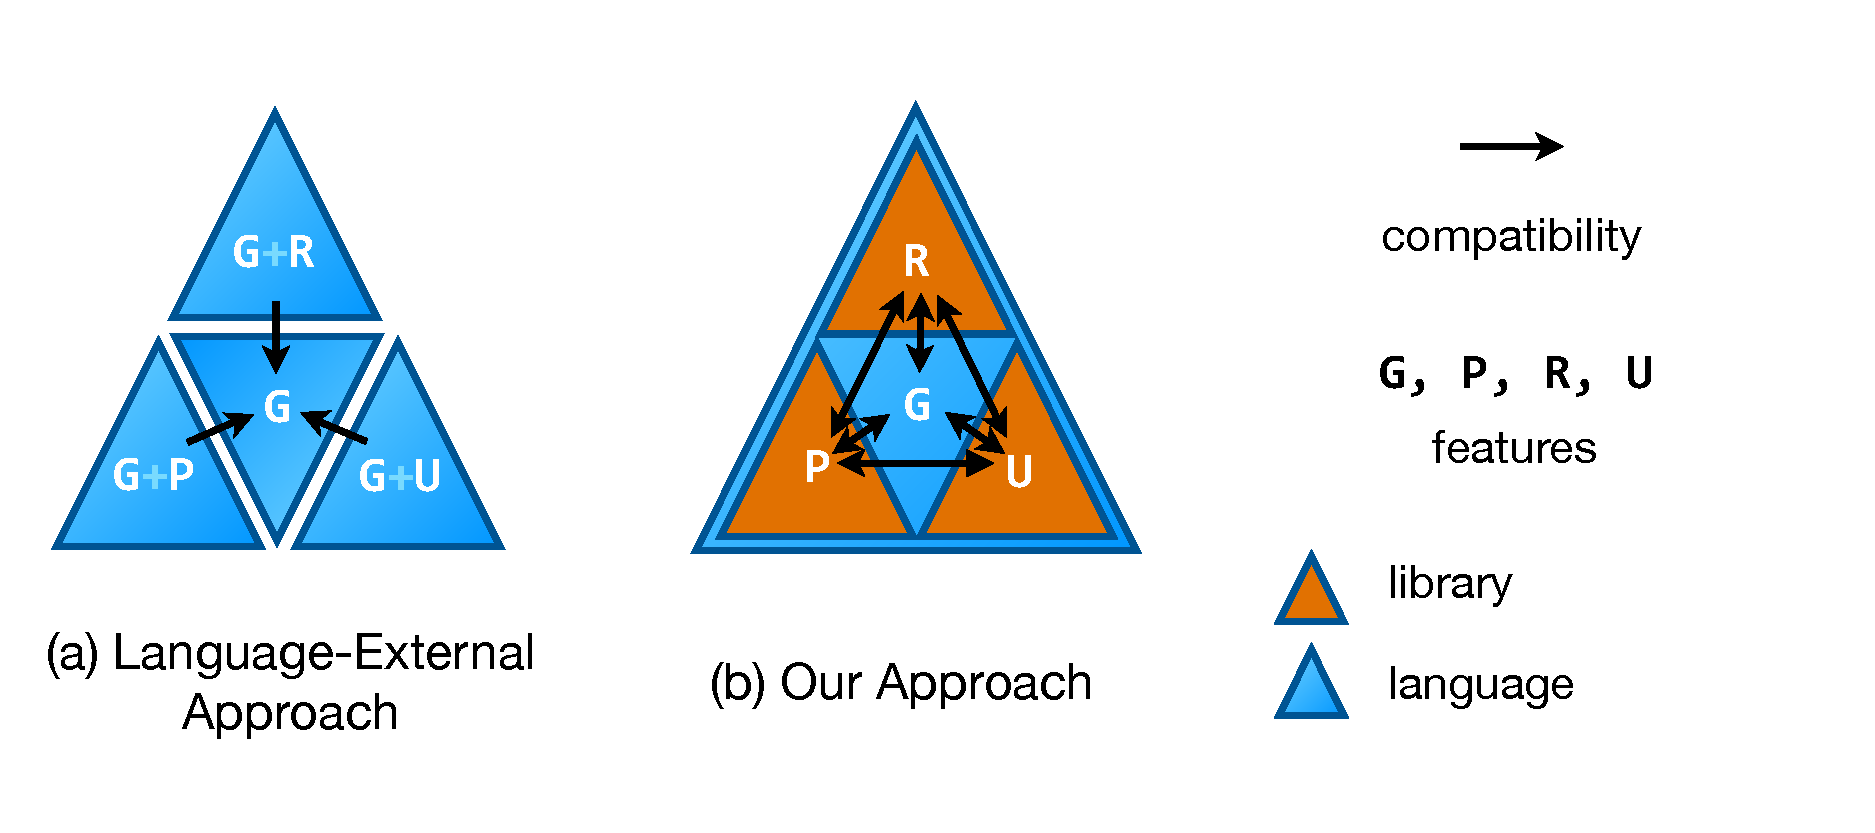
\includegraphics[scale=0.5]{approaches.pdf}
%\end{center}
%\vspace{-20px}
%\caption{\small (a) With a language-oriented approach, novel constructs are packaged into separate languages. Users can only safely and naturally call into languages consisting of common constructs (often only the common target language, such as C or Java bytecode). (b) With a language-internal extensibility approach, there is one system providing a common internal language, where additional primitive constructs that strictly strengthen its static guarantees or perform specialized code generation are specified and distributed within libraries. \label{approaches}}
%\end{figure*}

%As a result, domain-specific languages and new general-purpose abstractions alike have experienced relatively slow adoption in practice.
%
%Porting large codebases to new languages is difficult, and the dominant programming languages innovate slowly, so programming language.
%
%More specifically, such languages are neither \emph{internally extensible} because the language itself exposes only natural numbers and functions to its users, nor are they \emph{externally extensible} because no new behaviors can be added to the language's  implementation in a separate module from the one containing the initial implementation.

%This is the essence of a monolithic language implementation: it is impossible for anyone to modularly extend languages defined in this way. 


An extensible programming language could address these problems by providing a language-integrated mechanism for introducing new type and operator constructors and implementing their associated static and dynamic semantics. 
%Library developers need only consider which abstractions are most appropriate for their domain, without also considering whether these constructs can be exposed using abstractions appropriate to the domains of client code. Clients can simply import any necessary constructs when using a library that relies on them, preserving safety and ease-of-use without the use of  wrappers and glue code. We show this competing approach in Figure \ref{approaches}(b).
%Researchers and domain experts thus gain the ability to distribute new ideas for evaluation to a broader development community without requiring the approval of maintainers of mainstream languages, large-scale porting of code or explicit interoperability layers. 
But, as mentioned in Section \ref{language-integrated-approaches}, some significant challenges must be addressed before such a mechanism can be relied upon. The desire for expressiveness must be balanced against  concerns about maintaining various safety properties in the presence of arbitrary combinations of user-defined  extensions to the language's core semantics. The mechanism must ensure that desirable \emph{metatheoretic properties} (e.g. type safety, determinism, decidability) of the language are maintained by extensions. Because multiple independently developed extensions might be used within one program, the mechanism must further guarantee their \emph{non-interference}. These are the issues we seek to address in this work.
%\subsection{Theory}\label{atlam}
%%\begin{figure}
%%\begin{mathpar}
%%\inferrule{a}{b}
%%\end{mathpar}
%%\end{figure}
%In this section, we will describe a minimal calculus that captures our language-internal extensibility mechanism,  called \emph{active typechecking and translation (AT\&T)}. AT\&T allows developers to declare new primitive type families, associate operators with them, implement their static semantics in a functional style, and realize their dynamic semantics by simultaneously implementing a translation into a typed internal language. Note that this latter mechanism is closely related to how Standard ML was (re-)specified\todo{cite/read a bit about this/ask Bob/flesh this out}, but that we are fundamentally interested in extending language \emph{implementations}, not their  declarative specifications; proving the adequacy of such implementations against mechanized specifications, or extracting them directly from such specifications, will be investigated in future work.
%
%The AT\&T mechanism utilizes type-level computation of higher kind and integrates typed compilation techniques into the language to allow us to give strong metatheoretic guarantees,  and uses a mechanism notionally related to abstract types (such as those found in the ML module system) to guarantee that extensions cannot interfere with one another,  while remaining straightforward and expressive. In this section, we will develop a core calculus, called \atlam, which uses a minimal, uniform grammar for primitive operators. Then in Section \ref{ace}, we will show how to realize this minimal mechanism within a widely-used language with a more expressive grammar.
%
%AT\&T is general with respect to many choices about the type-level language, the typed internal language and syntax. Choices along these dimensions can affect both expressiveness and ease-of-use. We will begin in Sec. 2 by introducing a minimal system called $@\lambda$ (the ``actively-typed lambda calculus'') that distills the essence of the mechanism in a simply-typed, simply-kinded setting. This will allow us to fully and concisely formalize the language and compiler and give several key safety theorems. We will then continue in Sec. 3 by discussing variants of this mechanism based on other basic paradigms, considering dependently-typed functional languages and object-oriented languages, discussing trade-offs between expressivity and safety when doing so. We have developed a simple prototype called Ace and have used it to develop a number of full-scale language extensions as libraries. We will briefly discuss this language and these extensions in Sec. 4.

%We note at the outset that AT\&T focuses on extending the static semantics of languages with fixed, though flexible, syntax. Language-internal syntax extension mechanisms have been developed in the past (e.g. SugarJ \cite{sugarj}) but they have also suffered from safety problems because grammar composition is not always safe when done in an  unconstrained manner. Constrained approaches that provide stronger safety guarantees have recently been outlined (e.g. Wyvern \cite{globaldsl13}) but we will leave integration of syntax extensions with semantic extensions as future work.

\subsubsection{From Extensible Compilers to Extensible Languages}\label{evolution}
The monolithic character of most programming languages is reflected in, and perhaps influenced by, the most common techniques used for implementing programming languages. Programming languages are not implemented using open representations of types or expressions. 
Let us consider an implementation of the STLC. 
A compiler written using a functional language will invariably represent the primitive type  and operator constructors using {closed} recursive sums. 
A simple implementation in Standard ML may be based around these datatypes, for example:
\begin{lstlisting}
  datatype Type = Arrow of Type * Type
  datatype Exp = Var of var | Lam of var * Type * Exp | Ap of Exp * Exp 
\end{lstlisting}

The compiler front-end, which consists of a typechecker and translator to a suitable intermediate language (for subsequent compilation by some suitable back-end), will proceed by exhaustive case analysis over the constructors of \lstinline{Exp}.

In a class-based object-oriented implementation of Godel's T, we might instead encode type and operator constructors as subclasses of abstract classes \lstinline{Type} and \lstinline{Exp}. Typechecking and translation, however, will proceed by the ubiquitous \emph{visitor pattern}, dispatching against a fixed collection of {known} subclasses of \lstinline{Exp}.

In either case, we encounter the same basic issue: there is no way to modularly add new primitive type and operator constructors to \li{Type} and \li{Exp}, respectively, and provide implementations of their associated typechecking and translation logic. 
%This issue is related to the widely-discussed \emph{expression problem} (in a restricted sense -- we do not consider adding new functions beyond typechecking and translation here, only adding logic to these) \cite{wadler-expression}.

A number of language mechanisms have been proposed that allow new cases to be added to datatypes and the functions that operate over them in a modular manner. 
In functional languages, we might use \emph{open datatypes} \cite{opendatatypes}\todo{cite}. For example, if we wish to extend our implementation of the STLC with product types and we have written our compiler in a language supporting open inductive datatypes, it might be possible to add new cases: 
\begin{lstlisting}
  newcase Prod of Type * Type extends Type
  newcase Pair of Exp * Exp extends Exp
  newcase PrL of Exp extends Exp
  newcase PrR of Exp extends Exp
\end{lstlisting}

The logic for functionality like typechecking and translation can then be implemented for only these new cases. For example, the \lstinline{typeof} function that synthesizes a type for an expression given a context could be extended to support the new case \li{PrL} like so:
\begin{lstlisting}
  typeof (ctx, PrL(e)) = case typeof (ctx, e) of 
      Prod(t1, _) => t1 
    | _ => raise TypeError("<appropriate error message>")
\end{lstlisting}

If we allowed users to define new modules containing definitions like these and link them into our compiler, we will have succeeded in creating an externally-extensible compiler, albeit one where safety and non-interference is not guaranteed (we will return to this point shortly). We have not, however, created an extensible programming language because other compilers for the same language will not necessarily support the same extensions. 
If our newly-introduced constructs are exposed at a library's  interface boundary, clients of that library who are using different compilers face the same problems with client compatibility that those using different languages face (as described in Sec. \ref{external-approaches}). That is, {extending a language by extending a single compiler for it is morally equivalent to creating a new language}. 

We argue that a more appropriate and useful place for extensions like this is directly within libraries, alongside abstractions that can be implemented in terms of existing primitive abstractions. To enable this, the language must allow for the introduction of new type constructors, like \lstinline{Prod}, operator constructors, like \lstinline{Pair}, \lstinline{PrL} and \lstinline{PrR}, and their associated type synthesis and translation logic. Because this mechanism is integrated into the language, all compilers must support it to satisfy the language specification.

The design described above suggests we may now need to add another layer to our language, beyond the type-level language ($\tau$) and expression language ($e$) where extensions are implemented. In fact, we will show that \textbf{a natural place for type system extensions is within the type-level language}. The intuition  is that extensions to a statically typed language's semantics will need to manipulate types as values at compile-time. Many languages already allow users to write type-level functions for various reasons, effectively supporting this notion of types as values at compile-time. The type-level language is often constrained by its own type system, where the types of type-level terms are called \emph{kinds} for clarity,  that prevents type-level functions from causing problems during compilation. This is often more constrained than the expression language is (e.g. it might guarantee termination, to ensure that typechecking is decidable). This is precisely the structure that a distinct extension layer would have, and so it is quite natural to unify the two.


\subsubsection{@$\lambda$}
We will begin by developing an ``actively-typed'' version of the simply-typed lambda calculus with type-level computation called @$\lambda$. In the semantics for this calculus, we will integrate typed compilation techniques and a form of abstract types to allow us to prove key type safety and non-interference theorems. 

We specify the semantics of the external language as a Harper-Stone style elaboration semantics: all terms in the external language are simultaneously assigned a type and an elaboration to a term in a fixed typed internal language \cite{HarperStone}.  The mechanism will check that the elaboration is type preserving, following upon work done on the TIL compiler for Standard ML by Morrisett et al. \cite{TIL}, so that the semantics can be reasoned about compositionally and so that type safety can be proven. 

Any  global properties that the internal language maintains are guaranteed to hold no matter which extensions are used. In other words, extension providers cannot implement type systems weaker than the type system of the internal language. Providers are able to implement type systems stronger than the internal type system. We are interested in permitting only deterministic, decidable extensions, so semantic extensions are implemented as total functions in the type-level language (essentially, as a typechecker), rather than extracted from inductive specifications, like those in the Sec. \ref{foundations}\footnote{Though we will not explore this further in this thesis, a system for extracting such a function from a declarative specification could potentially be implemented using the techniques in Sec. \ref{aparsing} -- a \emph{kind-specific language}!}. This has the added benefit of giving providers finer-grained control over error messages -- with a strictly inductive specification, it is difficult to provide different error messages for different failure points in a derivation.
%In this section, we will sketch a calculus where new type families and operator families can be introduced by users. The type synthesis and translation logic that implements the desired static and dynamic semantics, respectively, for these is implemented in the type-level language. 

To give an example, the fragment in Fig. \ref{nat-atlam} shows how to introduce a new type constructor, \li{Nat}, indexed trivially (i.e. by a value of kind unit). Each type constructor must have a \emph{representation schema} associated with it that determines an associated internal type for every value  the index might take. The {representation schema} of $\fvar{Nat}$ is given on line 2 by a type-level function from the index to an internal type, $\mathbb{Z}$. Internal types, $\sigma$, are reflected into the type-level language, $\tau$, via the form $\blacktriangledown(\sigma)$. 

A key decision that we make is to associate operator constructors directly with type constructors. This provides a scope for information hiding, as we will discuss, and also forms the foundation for a higher-level  elaboration mechanism that allows us to use a more conventional (though still fixed) concrete syntax for expressions, rather than the uniform abstract syntax that the language as specified uses. We will explore this in the design of Ace. The definitions of three new operator constructors are given on lines 3-XXX\todo{finish this}. 

\begin{figure}
\begin{lstlisting}
tycon $\fvar{Nat}$ of unit with  
    schema $\lambda$idx:unit.$\blacktriangledown$($\mathbb{Z}$) 
    opcon Z of unit ($\lambda$idx:unit.$\lambda$args:list[Den].empty args [[$\triangledown$(0) as Nat[()]]])
    opcon S of unit ($\lambda$idx:unit.$\lambda$args:list[Den].pop_final args $\lambda$trans:ITm.$\lambda$ty:$\star$. 
      if ty = Nat[()] then [[$\triangledown$($\vartriangle$(trans)+1) as Nat[()]]] else err("...S requires nat..."))
    opcon Rec of unit ($\lambda$idx:unit.$\lambda$args:list[Den].pop args $\lambda$.a.a.a..aa.a)
end
\end{lstlisting}
\caption{An implementation of primitive natural numbers as internal integers in @$\lambda$.}
\label{nat-atlam}
\end{figure}



A draft of the full definition of this calculus is available as a paper draft\footnote{\url{https://github.com/cyrus-/papers/tree/master/esop14}}.


\subsection{Ace}\label{ace}
The syntax of @$\lambda$ is abstract -- there is a single uniform operator application form. To be practical, a wider variety of syntactic constructs must be used. A number of other practical considerations are also important. This section describes the design and implementation of Ace, an internally-extensible language designed considering both extrinsic and intrinsic criteria. To solve the bootstrapping problem, Ace is implemented entirely as a library within the popular Python programming language. Ace and Python share a common syntax and package system, allowing Ace to leverage its well-established tools and infrastructure directly. Python serves as the compile-time metalanguage for Ace, but Ace functions themselves do not operate according to Python's fixed dynamically-typed semantics  (cf. \cite{Politz:2013:PFM:2509136.2509536,python}). Instead, Ace has a statically-typed semantics that can be extended by users from within libraries. 

More specifically, each Ace function can be annotated with a base semantics that determines the meaning of simple expressions like literals and certain statements. The semantics of the remaining expressions and statements are governed by logic associated with the type of a designated subexpression. We call the user-defined base semantics \emph{active bases} and the types in Ace \emph{active types}, borrowing terminology from \emph{active libraries} (\cite{activelibraries}, see Sec. \ref{related}). Both are objects that can be defined and manipulated at compile-time using Python. An important consequence of this mechanism is that it permits \emph{compositional} reasoning -- active bases and active types govern only specific non-overlapping portions of a program. As a result, clients are able to import any combination of extensions with the confidence that link-time ambiguities cannot occur (unlike many previous approaches, as we discuss in Sec. \ref{related}).

The \emph{target} of compilation is also user-defined. We will show examples of Ace targeting Python as well as OpenCL, CUDA and C99, lower-level languages often used to program hardware. An active base or type can support multiple \emph{active targets}, which mediate translation of Ace code to code in a target language. Ace functions targeting a language with Python bindings can be called directly from Python scripts, with compilation occurring implicitly. For some data structures, types can propagate from Python into Ace. We show how this can be used to streamline the kinds of interactive workflows that Python is often used for. Ace can also be used non-interactively from the shell, producing source files that can be further compiled and executed by external means.

The remainder of the section is organized as follows: in Sec. \ref{usage}, we describe the basic structure and usage of Ace with an example library that internalizes and extends the OpenCL language. Then in Sec. \ref{att}, we show how this and other libraries are implemented by detailing the extension mechanisms within Ace. To explain and demonstrate the expressiveness of these mechanisms (in particular, active types) further, we continue in Sec.  \ref{examples} by showing a diverse collection of abstractions drawn from different language paradigms that can be implemented as orthogonal libraries in Ace. We include functional datatypes, objects, and several other abstractions.  A full paper draft is available\footnote{\url{https://github.com/cyrus-/papers/tree/master/ace-pldi14}}.

NOTE: Having an issue with tex macros but pretend sections 2-4 of the Ace paper are here basically as-is.

\subsection{Remaining Tasks}
\begin{itemize}
\item We need to fix a minor issue raised by a reviewer in the semantics of @$\lambda$ about variables in internal terms when they are substituted.
\item We need to write full proofs of the theorems stated in the @$\lambda$ paper.
\item We need to develop an elaboration of a subset of the Python grammar to @$\lambda$, to connect the two.
\item We need to detail the examples in Sec. 4 of the Ace paper more substantially.
\end{itemize}
